% !TEX root = Simulation.tex

\chapter{DNA Computing - Text Chapter 9}

Most of this section of the assignment was paraphrased or expanded on from Wikipedia articles.

\section{Problem 1}
\textbf{
Name four problems that cannot be solved by a Turing machine.
}

\hfill \\

\begin{description}
\item Halting Problem
\item Determining a busy beaver\footnote{"Busy Beaver" is my favorite program name of all time.} champion
\item The Mortality Problem
\item Determining whether a given machine computes a partial function with a nontrivial property of partial functions.
\end{description}


\section{Problem 2}
\textbf{
Name four NP-complete and four NP-hard problems.
}

\hfill \\

\begin{minipage}[b]{.5\hsize}
	\centerline{\textbf{NP-complete problems}}
	\begin{description}
	\item{SAT problem}
	\item{Hamiltonian Path Problem (HPP)}
	\item{Knapsack Problem}
	\item{Partition Problem}
	\end{description}
\end{minipage}	
\begin{minipage}[b]{.5\hsize}
	\centerline{\textbf{NP-hard problems}}
	\begin{description}
	\item{Subset Sum Problem}
	\item{Traveling Salesman Problem}
	\item{K Minimum-spanning tree}
	\item{Graph Coloring Problem}
	\end{description}
\end{minipage}


\newpage
\section{Problem 5}
\textbf{
The two most basic DNA sequencing techniques are known as a) Maxam-Gilbert and b) Sanger, after their proponents. Explain how each of these techniques work and contrast them.
}

\hfill \\

\begin{description}
\item{\textbf{Maxam-Gilbert Sequencing}} \hfill \\
Maxam-Gilbert Sequencing works by cleaving the DNA strands via four different solutions. The solutions are balanced in such a way that each strand will, on average, only be cleaved once. The four solutions cleave at different deoxynucleotides: (A + G), G, C, \& (C + T).

After electrophoresing the leftover strands to sort them by size, you are left with a distribution of sizes in each solution. Reading these from shortest to longest, you can infer the deoxynucleotide at that position. Note: in the case of the (A + G) and (C + T) bands, the presence of A and T are infered by that band showing and a lack of the G and C bands respectively. An example graphic of Maxam-Gilbert Sequencing can be seen in Figure~\ref{sequencing} (a).

\item{\textbf{Sanger Sequencing}} \hfill \\
Sanger Sequencing clones a sequence of DNA in four different solutions. Each solution contains 3 of the normal deoxynucleotides that make up DNA chains. The fourth deoxynucleotide is replaced with a corresponding \textit{di}-deoxynucleotide which inhibits chaining due to it's lack of a 3'-OH group used to form phosphodiester bonds. The di-deoxynucleotides can be labeled through various methods including florescence or radioactivity.

Once the DNA is copied, the four strands are heat denatured and separated by length using gel electrophoresis. The length of the strands was limited by the di-deoxynucleotide which means the different lengths of the strands in each solution corresponds to places where the corresponding deoxynucleotide would reside. The sequence can then be read by reading the relative positions in the four lanes. An example of this type of sequencing can be found in Figure~\ref{sequencing} (b).

\end{description}

\begin{figure} 
\centering
\begin{tabular}{ c c c }
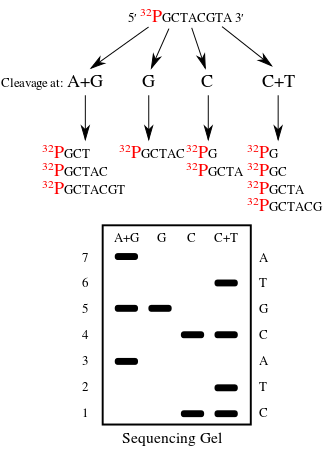
\includegraphics[scale=.75]{MaxamGilbertSequencing} & \hspace{10pt} &
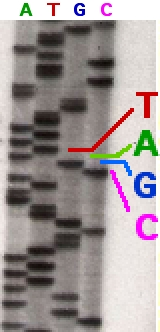
\includegraphics{SangerSequencing} \\
(a) &  & (b)
\end{tabular}
\caption[DNA Sequencing Methods]{DNA Sequencing Methods. (a)Maxam-Gilbert Sequencing (b)Sanger Sequencing}
\label{sequencing}
\end{figure}

